%% main_v3.tex — CIKM '26 camera-ready rewrite (revision 2)
%% Style modeled on CIKM '25 published papers (e.g., DIVERS, SUMMA, HEN).
%% Revision 2: gap-first narrative; explicit RQs+H1/H2/H3; gap-aligned Related Work;
%%             citation-backed claims; surfaced methodology numbers; multi-LLM bias control;
%%             reframed structural-compliance claims; explicit agentic-RAG comparison.

\documentclass[sigconf, anonymous]{acmart}

%% ---- ACM rights / conference info ----
%% SUBMISSION STAGE: ACM Reference Format and copyright footnote are
%% suppressed below because real DOI/ISBN are assigned by ACM only after
%% acceptance. AT CAMERA-READY: uncomment the macros below, replace the
%% X-placeholders with ACM-issued values, and remove the three suppression
%% lines that follow. The block will then auto-display in the camera-ready PDF.
%
% \setcopyright{acmlicensed}
% \copyrightyear{2026}
% \acmYear{2026}
% \acmConference[CIKM '26]{Proceedings of the 35th ACM International Conference on Information and Knowledge Management}{November 9--13, 2026}{Atlanta, GA, USA}
% \acmBooktitle{Proceedings of the 35th ACM International Conference on Information and Knowledge Management (CIKM '26), November 9--13, 2026, Atlanta, GA, USA}
% \acmPrice{15.00}
% \acmDOI{10.1145/XXXXXXX.XXXXXXX}
% \acmISBN{979-8-4007-XXXX-X/26/11}

%% Suppression for submission/review stage
\settopmatter{printacmref=false}
\renewcommand\footnotetextcopyrightpermission[1]{}
\pagestyle{plain}
%% Override the acmart default page-header placeholder
%% ("Conference'17, July 2017, Washington, DC, USA") with anonymous CIKM '26
%% submission text. Venue/date are public conference info, not identity-revealing.
\acmConference[CIKM '26 Submission]{Anonymous Submission to CIKM '26}{November 2026}{Atlanta, GA, USA}

%% ---- packages ----
\microtypesetup{expansion=false}
\usepackage[T1]{fontenc}
\usepackage{booktabs}
\usepackage{graphicx}
\usepackage{amsmath}
\let\Bbbk\relax
\usepackage{amssymb}
\usepackage{xcolor}
\usepackage{url}
\usepackage{float}
\usepackage{placeins}
\usepackage{caption}
\usepackage{longtable}
\usepackage{tabularx}
\usepackage{array}
\usepackage{calc}
\usepackage{tikz}
\usetikzlibrary{positioning,arrows.meta}
\providecommand{\tightlist}{\setlength{\itemsep}{0pt}\setlength{\parskip}{0pt}}
\renewcommand{\topfraction}{0.9}
\renewcommand{\bottomfraction}{0.8}
\renewcommand{\textfraction}{0.07}
\renewcommand{\floatpagefraction}{0.7}
\raggedbottom
\emergencystretch=3em
\hyphenpenalty=50
\tolerance=1000
\setlength{\tabcolsep}{3pt}
\hyphenation{re-pro-duc-tion spec-i-fi-ca-tions knowledge-graph-grounded
 taxonomy-grounded An-ten-na-Pod New-Pipe Thun-der-bird
 con-fi-dent cleanlab hi-er-ar-chi-cal cov-er-age IssueSpec}

%% ---- Compactness tweaks (review-stage; ACM-compatible: no \section redef) ----
\usepackage{enumitem}
\setlist{itemsep=1pt, topsep=2pt, parsep=0pt, leftmargin=1.2em}
\setlength{\textfloatsep}{6pt plus 1pt minus 1pt}
\setlength{\intextsep}{6pt plus 1pt minus 1pt}
\setlength{\dbltextfloatsep}{6pt plus 1pt minus 1pt}
\setlength{\floatsep}{6pt plus 1pt minus 1pt}
\setlength{\abovecaptionskip}{3pt}
\setlength{\belowcaptionskip}{0pt}
\setlength{\parskip}{0pt}
\setlength{\itemsep}{0pt}

\begin{document}

\title[IssueSpec]{\large IssueSpec: A Framework for Structured Review-to-Issue Translation}

%% Anonymous author block for submission/review. The `anonymous` documentclass
%% option also auto-anonymizes any author info if uncommented elsewhere.
%% At camera-ready: remove `anonymous` from \documentclass and replace the
%% block below with real author info.
\author{Anonymous Author(s)}
\email{anonymous@example.com}
\affiliation{%
 \institution{Anonymous Institution}
 \city{Anonymous City}
 \country{Anonymous Country}}

\renewcommand{\shortauthors}{Anonymous}

\begin{abstract}
  App developers daily receive millions of noisy reviews, reporting bugs, feature requests,
  performance issues, and device-specific problems. Manual review and triage cannot scale, and
  defect trackers such as JIRA require structured fields (steps to reproduce, severity, and
  component) rather than free text. Classifiers predict an issue label like ``bug'' or ``feature
   request'' but leave the remaining structured fields unaddressed. Response generators emit
  user-facing replies without explicitly identifying the underlying defect. Agentic
  software-engineering tools generate code patches from well-formed issue specifications, not
  from noisy review text. Knowledge graph tools cluster reviews by topic and produce free-form
  summaries rather than typed structured fields. Reinforcement Learning from Human Feedback
  (RLHF), which aligns Large Language Model (LLM) outputs with human preferences via pairwise
  comparisons, has been applied to general-safety settings but not to the multi-constraint
  compliance required for structured review-to-issue translation. We propose \textbf{IssueSpec},
   a framework for structured review-to-issue translation built around a typed Intermediate
  Representation (IR) that converts each noisy review into one of five predefined report types
  (Zimmermann bug reports, Cohn user stories, ISO/IEC~25010 non-functional categories, Nielsen
  usability heuristics, and device-OS compatibility matrices). The framework combines
  knowledge-graph clustering for contextual grouping, a verified-anchor procedure for noise
  correction, the \textsc{SpecCov} metric for faithfulness validation, and a Constrained Markov
  Decision Process (CMDP)-based alignment trainer for downstream response generation under
  quality and compliance constraints. We evaluate the framework on 215{,}583 reviews from 58
  Android apps; on a stratified  28-spec subsample, it achieves $3.89/5$ on a five-dimension issue-specification rubric. When
  these validated IssueSpecs are used as input to Retrieval-Augmented Generation (RAG),
  human-rated response quality improves by $+2.36$ Likert points over retrieval alone (5-point
  scale, $n=100$ paired comparisons from a 400-row blinded rating set, $p<0.001$), consistent across four LLMs from three model
  families. We release the IssueSpec schema, large-scale benchmark dataset, \textsc{SpecCov}
  faithfulness metric, verified-anchor resource, and a CMDP-based RLHF testbed to support future
   research on structured information extraction and constrained generation.
  \end{abstract}
%% ---- CCS Concepts ----
\begin{CCSXML}
<ccs2012>
  <concept>
    <concept_id>10010147.10010178.10010179</concept_id>
    <concept_desc>Computing methodologies~Natural language processing</concept_desc>
    <concept_significance>500</concept_significance>
  </concept>
  <concept>
    <concept_id>10002951.10002952.10003219</concept_id>
    <concept_desc>Information systems~Information extraction</concept_desc>
    <concept_significance>300</concept_significance>
  </concept>
  <concept>
    <concept_id>10011007.10011074.10011099</concept_id>
    <concept_desc>Software and its engineering~Software maintenance tools</concept_desc>
    <concept_significance>300</concept_significance>
  </concept>
  <concept>
    <concept_id>10010147.10010257.10010293.10010294</concept_id>
    <concept_desc>Computing methodologies~Reinforcement learning</concept_desc>
    <concept_significance>100</concept_significance>
  </concept>
</ccs2012>
\end{CCSXML}

\ccsdesc[500]{Computing methodologies~Natural language processing}
\ccsdesc[300]{Information systems~Information extraction}
\ccsdesc[300]{Software and its engineering~Software maintenance tools}
\ccsdesc[100]{Computing methodologies~Reinforcement learning}

\keywords{App Reviews, Knowledge Graph, Intermediate Representation, Retrieval-Augmented Generation, RLHF, Software Engineering, Issue Tracking}

\maketitle

%% =====================================================================
\section{Introduction}\label{introduction}

App stores are where users talk back to developers. A single popular app pulls in thousands of reviews a week, and the global stream runs into millions a day~\cite{maalej2016, gao2019rrgen, dabrowski2022analysing}. These reviews carry the signals developers need to act on: bug reports (a crash on Samsung S8 after an update), feature requests (dark mode), performance complaints (battery drain), and regression notes (voice search no longer works). The information is real, but it shows up as messy free-form text, usually without the details required to reproduce a bug or scope a new feature.

To turn any of this into work, developers rely on defect trackers such as JIRA or GitHub Issues. Those tools, though, can't work with raw text; they need structured fields such as issue type, steps to reproduce, severity, and affected component~\cite{chaparro2017detecting,
zimmermann2010}. Filling those fields by hand does not scale with the volume modern apps face. Years of work on automated review pipelines has helped with the surrounding tasks like classification, summarization, and response generation, but no system actually produces the structured report a developer can paste directly into a tracker. D{\k a}browski et al.'s nineteen-year survey of the field~\cite{dabrowski2022analysing} confirms the same boundary.

Prior work has tackled several pieces of this problem separately.
  Classifiers~\cite{maalej2016, chen2014arminer, villarroel2016, disorbo2016surf} take a review
  and predict an issue label such as bug or feature request. Response
  generators~\cite{gao2019rrgen, gao2020core, lewis2020rag} produce a polite reply for the user.
   Agentic software-engineering tools such as SWE-Agent~\cite{yang2024sweagent} and
  RepairAgent~\cite{bouzenia2024repairagent} take a clean GitHub issue and generate a code
  patch. Knowledge-graph methods~\cite{xu2025reviewgraph, kgcpn2023, keertipati2016} cluster
  reviews into themes or surface frequent complaints. Each of these has matured over the past
  decade and works well within its own scope.



But none of these reaches the developer-ready issue report a defect tracker needs. The
  Maalej-Nabil classifier taxonomy~\cite{maalej2016} and its successors~\cite{chen2014arminer,
  villarroel2016, disorbo2016surf, kaur2023bertrcnn, shah2021reviewmining} have settled at an F1
   ceiling around 0.75--0.85, a label-quality limit (not a model-capacity one) per D{\k
  a}browski et al.'s~\cite{dabrowski2022analysing} nineteen-year survey. The label is only the
  first piece of what a tracker entry needs; the remaining fields (steps to reproduce, severity,
   affected component) have to come from somewhere, and classification-only pipelines leave that
   downstream step to manual triage. Response generators like RRGen~\cite{gao2019rrgen} and
  CoRe~\cite{gao2020core} address the customer-communication side of the workflow, but the
  actual bug behind the review is never written out in the structured form a tracker needs, so
  even a perfect reply system does not give developers something they can paste into JIRA.
  Agentic SE tools assume a well-formed bug report or GitHub issue as the agent's starting
  state, built into the SWE-bench protocol~\cite{jimenez2024swebench} where each instance is a
  (GitHub issue, code repository) pair; constructing such an issue from raw review text is
  explicitly outside the protocol, leaving the upstream gap unaddressed.

Knowledge-graph methods stop at intermediate outputs rather than typed fields:
  ReviewGraph~\cite{xu2025reviewgraph}, KGCPN~\cite{kgcpn2023}, and Keertipati et
  al.~\cite{keertipati2016} each output rating predictions, summaries, or feature rankings, none
   of which a defect tracker can ingest directly. RLHF has matured into the standard approach
  for aligning LLM outputs with human preferences (DPO~\cite{rafailov2023},
  KTO~\cite{ethayarajh2024}, PPO~\cite{schulman2017ppo}), and Safe-RLHF~\cite{dai2023} extends
  the framework to multi-objective settings under a Constrained MDP for general LLM safety
  (harmfulness, dishonesty, bias). The developer-relations setting poses a different question
  entirely: how to align responses under a domain-specific constraint family (truthful promises,
   no information leakage, professional tone, legal-safe wording) rooted in business and legal
  exposure. To our knowledge, no published RLHF formulation has been adapted to this constraint
  set.

This work pursues three aims. First, we develop a framework that turns noisy app reviews into structured, taxonomy-grounded issue specifications a defect tracker can consume directly. Second, we build a response generator that uses these specifications as input, producing replies that reference the actual underlying defect rather than generic templates. Third, we close the loop with a dual-objective alignment trainer that jointly optimizes for response helpfulness and the domain-specific compliance constraints of the developer-relations setting.

These aims map to three research questions.

\textbf{RQ1 (Translation Quality).} Can a typed IR, generated via a three-layer framework (knowledge-graph construction, hierarchical clustering,
standardized schema mapping), produce issue specifications that match or exceed the substantive completeness of human-written GitHub issues?

\textbf{RQ2 (Downstream Load-Bearing).} Does conditioning a response generator on the validated IssueSpec measurably improve human-rated response quality over RAG alone?

\textbf{RQ3 (Dual-Objective Alignment).} Can a CMDP-grounded RLHF loop progressing through KTO, DPO, and Constrained PPO jointly optimize response helpfulness and policy compliance for the
developer-relations setting?

To address these challenges, we propose \textbf{IssueSpec}, a framework for structured review-to-issue translation. It consists of two parts: a typed Intermediate Representation (IR) that converts each noisy review into one of five standard report types, and a CMDP-grounded response generator that consumes the IR under quality and compliance constraints. Figure \ref{fig:architecture} shows the full five-stage pipeline.

The main contributions of this work, each mapped to the gaps above, are:

\begin{itemize}\setlength{\itemsep}{2pt}
  \item \textbf{We propose} \textbf{IssueSpec}, the first typed Intermediate Representation (IR) for review-to-issue translation: a typed dictionary routed by issue class to one of five SE-taxonomy templates with verified standards-body provenance~\cite{zimmermann2010, cohn2004user, iso25010, nielsen1994, joorabchi2013real}.

  \item \textbf{We introduce} \textsc{SpecCov}, a stand-alone extractive-coverage faithfulness metric grounded in news-summarization practice~\cite{grusky2018newsroom,
  maynez2020faithfulness, kryscinski2020factcc}, together with a verified-anchor pipeline using confident learning~\cite{northcutt2021cleanlab} that lifts Cohen's $\kappa$ from $0.163$ to $0.592$ with 88.66\% independent classifier endorsement of corrections across 40{,}291 cases.
  
  \item \textbf{We design} a three-layer aspect-grounded knowledge graph that produces and prioritizes IssueSpecs via dependency-parsed aspect mining~\cite{hu2004mining},
  sentence-embedding-based clustering~\cite{reimers2019sentencebert, mcinnes2018umap,
  mcinnes2017hdbscan}, and PageRank centrality~\cite{page1999pagerank, brin1998anatomy}; the top-five aspects cover 74\% of all review-aspect mentions, roughly $10^3\times$ concentration in the developer's reading order.

  \item \textbf{We evaluate} the framework end-to-end on 215{,}583 reviews from 58 Android apps: IssueSpec achieves $3.89/5$ on a five-dimension issue-specification rubric, and adding it to RAG lifts human-rated response quality by $+2.36$ Likert points on 400 paired ratings ($p<0.001$), while retrieval alone is statistically indistinguishable from a no-context baseline; a four-LLM cross-family replication (Section~\ref{exp1-results}) rules out single-model bias.  

  \item \textbf{We release} a CMDP-grounded RLHF testbed (KTO~\cite{ethayarajh2024} to
  DPO~\cite{rafailov2023} to Lagrangian Constrained PPO~\cite{schulman2017ppo, dai2023}), formulated as a Constrained Markov Decision Process~\cite{altman1999, dai2023} that separates quality reward from compliance constraints, together with a benchmark dataset of 100 stratified clusters, a 490-review classification gold standard, 400 paired ratings, and a 99-review three-rater Krippendorff $\alpha = 0.451$ subsample.
  \end{itemize}
Table~\ref{tab:c2evidence} maps each contribution to its measurable headline result and
  released artifact. Figure \ref{fig:architecture} shows the five-stage
pipeline. 

\begin{table}[!htbp]\centering\footnotesize
\caption{Contribution-to-evidence-to-artifact map. Each contribution states a measurable headline result, the table or section that anchors it, and the named artifact released with this paper.}\label{tab:c2evidence}
\begin{tabular}{@{}p{1.5cm}p{3.0cm}p{2.9cm}@{}}\toprule
contribution & headline evidence & released artifact \\\midrule
IssueSpec & 0.96 template-fill vs 0.53 GitHub (Table~\ref{tab:stage3}); 5-dim rubric 3.89/5 (Table~\ref{tab:rubric}) & type-routed schema (Table~\ref{tab:templates}); \textsc{SpecCov} extractive-coverage scorer \\
IR load-bearing & $+2.36$ full vs \texttt{no\_spec} on 400 paired (Table~\ref{tab:stage4-human}); \texttt{no\_spec} indistinguishable from prompt baseline & 400 blinded paired ratings + 30-pair second-rater subset \\
verified anchor & $\kappa$ 0.16$\to$0.59 (Table~\ref{tab:kappa}); per-class F1 recovery
  (Table~\ref{tab:perclass-f1}); 88.66\% V5 endorsement on 40{,}291 cases & 5{,}230-review
  verified anchor + cleanlab correction procedure + V5 classifier \\
KG prioritization & $5.4\times$ lower Davies-Bouldin (Table~\ref{tab:cluster-quality}); top-5 PageRank aspects cover 74\% of mentions; count-controlled A1b (\S\ref{ablations}) & three-layer KG construction + count-controlled A1b output \\
CMDP RLHF + benchmark & constrained-proxy $+52\%$ BLEU-1 over SFT base (\S\ref{exp3-results});
   satisfied-at-init compliance scorer & CMDP formulation, KTO/DPO/constrained-proxy/CPPO
  trainers, benchmark (100 clusters, 400 ratings, 490 gold, $\alpha=0.451$ subsample) \\
\bottomrule\end{tabular}\end{table}

 \begin{figure*}[t]\centering
  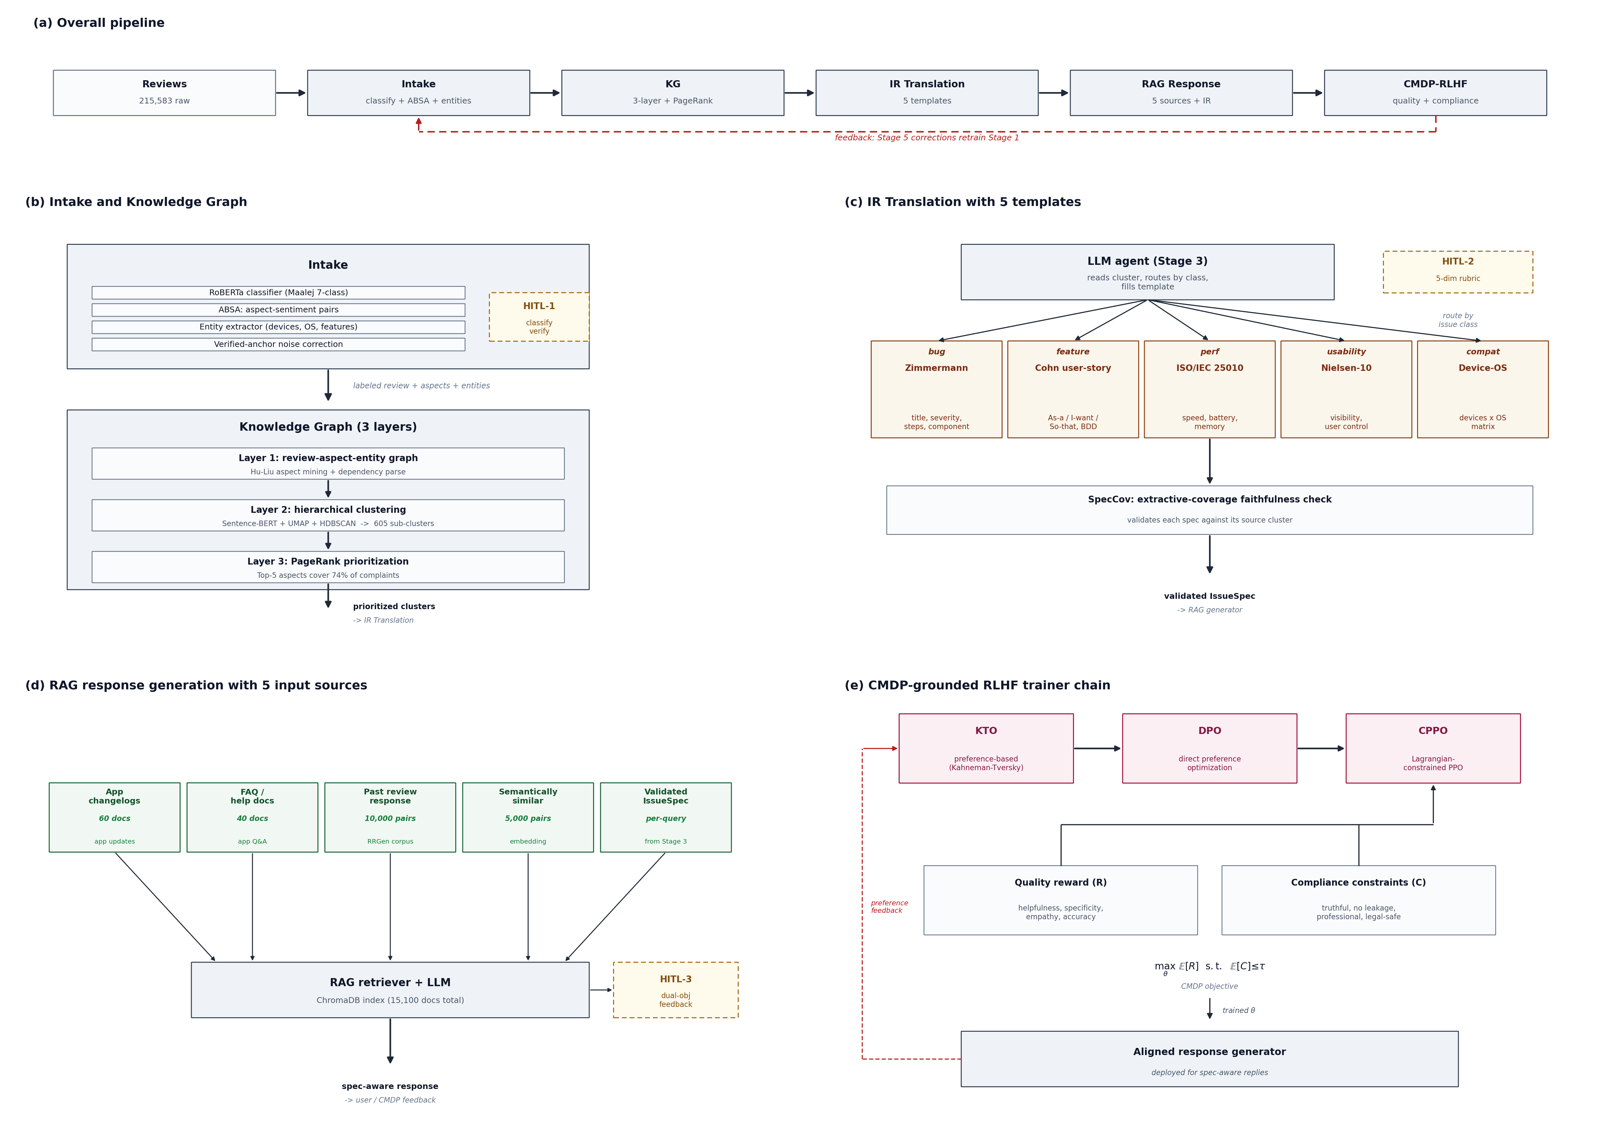
\includegraphics[width=\textwidth]{fig1_architecture.png}
  \caption{The IssueSpec architecture across four panels. \textbf{(b)} Intake (RoBERTa
  classifier, ABSA, entity extraction, verified-anchor noise correction) followed by the
  three-layer knowledge graph (review-aspect graph, hierarchical clustering, PageRank
  prioritization). \textbf{(c)} IR translation: the LLM agent routes each cluster to one of five
   standards-body templates (Zimmermann, Cohn, ISO/IEC~25010, Nielsen, device-OS) and the output
   is validated by \textsc{SpecCov}. \textbf{(d)} RAG response generation conditions on five
  fixed sources (changelogs, FAQ, past pairs, semantic neighbors, IssueSpec) over the ChromaDB
  index. \textbf{(e)} CMDP-grounded RLHF trainer chain (KTO~$\to$~DPO~$\to$~Constrained PPO)
  jointly optimizes a quality reward and four compliance constraints. HITL checkpoints (yellow,
  dashed) follow the selective prediction protocol~\cite{geifman2017selective,
  bansal2019}.}\label{fig:architecture}
  \end{figure*}
%% =====================================================================
\section{Related Work}\label{related-work}

We organize related work by the five gaps identified in Section~\ref{introduction}, naming what each field does, what assumption breaks for review-to-issue translation, and how IssueSpec differs.

\subsection{App Review Classification and Mining}
Maalej and Nabil~\cite{maalej2016} established the canonical seven-class taxonomy for app reviews. Subsequent systems, AR-Miner~\cite{chen2014arminer}, CLAP~\cite{villarroel2016}, SURF~\cite{disorbo2016surf}, BERT/RCNN hybrids~\cite{kaur2023bertrcnn, shah2021reviewmining}, and per-aspect sentiment analysis~\cite{guzman2014}, refined classification accuracy and added aspect-level granularity. Dąbrowski et al.~\cite{dabrowski2022analysing} surveyed nineteen years of such work and concluded that label quality, not model capacity, is the F1 ceiling at 0.75--0.85, an observation we corroborate in Section~\ref{exp1-results}. \emph{What breaks for review-to-issue translation:} none of these systems emits a typed developer-routable artifact downstream of the classification label. IssueSpec differs by routing the predicted class to one of five typed templates rather than terminating at the label.

\subsection{Response Generation and Retrieval-Augmented Generation}
RRGen~\cite{gao2019rrgen} and CoRe~\cite{gao2020core} pioneered end-to-end neural response generation on (review, response) pairs without an explicit structured intermediate. Vanilla RAG~\cite{lewis2020rag} retrieves relevant past responses in a single pass. \emph{Agentic RAG} variants, Self-RAG~\cite{asai2024selfrag} and DEMONSTRATE-SEARCH-PREDICT (DSP)~\cite{khattab2022demonstrate}, introduce iterative critique-revise loops that, in principle, could close the structured-intermediate gap. \emph{What breaks for review-to-issue translation:} none of these systems names the underlying defect, and our $n=10$ feasibility study (Section~\ref{exp2-results}) shows that agentic iteration without a typed intermediate adds modest gains (0.58$\to$0.70 rule-based score) compared with the $+2.36$ Likert-point gain from adding the IssueSpec. IssueSpec differs by injecting the typed intermediate as a first-class RAG source alongside retrieved past responses.

\subsection{Agentic Software Engineering}
SWE-Agent~\cite{yang2024sweagent}, RepairAgent~\cite{bouzenia2024repairagent}, and HyperAgent~\cite{phan2024hyperagent} consume well-structured GitHub issues to produce code patches through multi-step planning and tool use. \emph{What breaks for review-to-issue translation:} the issue specification is the input contract for all three systems; how a defect-tracker entry is constructed from noisy user-facing text is out of scope. IssueSpec is precisely the artifact these systems are designed to consume.

\subsection{Knowledge Graphs for App Reviews and Software Engineering}
Knowledge graphs have been used in software engineering for bug localization, report deduplication, and code understanding, but the issue specification is invariably treated as input rather than output. For app reviews specifically, ReviewGraph~\cite{xu2025reviewgraph} learns KG embeddings for rating prediction, KGCPN~\cite{kgcpn2023} produces KG-based extractive summaries, and Keertipati et al.~\cite{keertipati2016} apply graph centrality for coarse feature prioritization. \emph{What breaks for review-to-issue translation:} none of these systems maps KG nodes to a typed, developer-actionable issue schema, and no prior KG work has been applied to the specific task of producing GitHub-issue-quality artifacts from review text. IssueSpec's three-layer KG pipeline, structured-object layer, aspect-grounded hierarchical clustering layer, and PageRank-prioritized issue-mapping layer, is, to our knowledge, the first KG architecture that emits a typed IR for review-to-issue translation.

\subsection{RLHF and Constrained Optimization for Response Generation}
DPO~\cite{rafailov2023}, KTO~\cite{ethayarajh2024}, and PPO~\cite{schulman2017ppo} compress quality and compliance signals into a single scalar reward. Altman's CMDP framework~\cite{altman1999} separates these objectives, and Safe-RLHF~\cite{dai2023} applies CMDP to general LLM safety with a domain-agnostic compliance set covering harmful, dishonest, and biased outputs. \emph{What breaks for review-to-issue translation:} no prior work applies CMDP to dev-rel response generation, where the compliance set is domain-specific (promise safety, information leakage, tone guidelines, and legal safety). Our Stage~5 formulation differs by instantiating these four domain-specific constraints inside the CMDP Lagrangian and releasing a proof-of-concept training loop.

\subsection{Cross-Category Positioning}
Table~\ref{tab:cross-category} positions IssueSpec against representative prior systems across the five pipeline stages. Existing systems occupy at most two of the five stages; composing all five with a standardized issue schema, three theoretically-grounded HITL checkpoints, KG-centrality prioritization, and a CMDP-grounded RLHF formulation is the structural contribution of this work.

\begin{table*}[t]
  \centering
  \footnotesize
  \setlength{\tabcolsep}{4pt}
  \caption{Cross-category positioning. Existing systems compose at most two of the five pipeline
   stages. IssueSpec is the first to compose all five with a standardized issue schema, three
  HITL checkpoints grounded in selective prediction theory, KG-centrality prioritization, and a
  CMDP-grounded RLHF formulation. ``--'' denotes a stage absent from that system.}
  \label{tab:cross-category}
  \begin{tabular}{lccccc}
  \toprule
  System & Classify & Cluster & IssueSpec & Response & RLHF \\
  \midrule
  AR-Miner~\cite{chen2014arminer} & filter & LDA topic & -- & -- & -- \\
  CLAP~\cite{villarroel2016} & rating & DBSCAN & -- & -- & -- \\
  SURF~\cite{disorbo2016surf} & intention & LDA & -- & summary & -- \\
  RRGen~\cite{gao2019rrgen} & -- & -- & -- & seq2seq & -- \\
  CoRe~\cite{gao2020core} & -- & -- & -- & context-aware retrieval & -- \\
  Maalej~\cite{maalej2016} & 7-class & -- & -- & -- & -- \\
  ReviewGraph~\cite{xu2025reviewgraph} & rating & KG & -- & -- & -- \\
  SWE-Agent~\cite{yang2024sweagent} & -- & -- & consumes (not produces) & -- & -- \\
  Safe-RLHF~\cite{dai2023} & -- & -- & -- & general & dual-CMDP (general) \\
  \textbf{IssueSpec (ours)} & \textbf{V5 corrected} & \textbf{KG + PageRank} &
  \textbf{type-routed schema} & \textbf{spec-aware RAG} & \textbf{dual-CMDP (dev-rel)} \\
  \bottomrule
  \end{tabular}
  \end{table*}

%% =====================================================================
\section{The IssueSpec Pipeline}\label{system-design}

The IssueSpec pipeline (Fig.~\ref{fig:architecture}) is a five-stage information-extraction cascade~\cite{hearst1999, sarawagi2008}. Stages~1--3 produce the typed IR from raw reviews; Stage~4 uses it to drive spec-aware response generation; Stage~5 aligns the response generator via constrained RLHF. We describe each stage in turn, with the verified-by-citation taxonomy templates in Table~\ref{tab:templates}.

\subsection{Producing the IR}\label{aim1}

\textbf{Stage 1: Intake, Classification, and Aspect Extraction.}
  Stage~1 produces three outputs per review: a multi-label class from a
  RoBERTa head fine-tuned on Maalej~\cite{maalej2016} and
  Guzman~\cite{guzman2014} (reviews often mix concerns, like a bug
  report that also asks for a feature); aspect-level
  sentiment~\cite{guzman2014} so ``great UI but terrible battery'' is
  kept as separate pairs rather than averaged to a star rating; and
  entity extraction for devices, OS versions, and named features, which
  the Stage~3 device-OS and bug-report templates need as typed fields.
  Low-confidence reviews route to HITL-1 under selective-prediction
  theory~\cite{geifman2017selective}: when the classifier cannot decide,
  the expert does, and the correction feeds the next training round.

  LLM annotation noise is the main challenge here. On the
  5{,}041-review praise stratum, 25\% of LLM labels are wrong,
  concentrated on minority classes. Discarding them wastes annotation;
  using them as-is poisons training. We apply confident
  learning~\cite{northcutt2021cleanlab} against a verified anchor of
  5{,}230 expert-labeled reviews plus 5{,}008 from
  Maalej~\cite{maalej2016}, gated by anchor confidence $\geq 0.70$ and
  LLM probability $\leq 0.20$; this keeps the good labels and corrects
  only the wrong ones. The compatibility class needs a separate fix:
  only 8 of 215{,}583 LLM labels are tagged \texttt{compatibility}, and
  Maalej has none. We seed it with 200 synthetic reviews from device,
  OS, and screen templates~\cite{joorabchi2013real}, plus 100 mined from
  RRGen via compatibility keywords, each checked by the lead author
  before training.
  
  \textbf{Stage 2: Three-Layer Knowledge Graph.} Stage~2 organizes
  reviews into an aspect-grounded knowledge graph: build, cluster,
  prioritize. The first layer builds the graph: each review is a node
  linked to its aspects and entities by sentiment and temporal edges. A
  graph beats a flat list because reviews share aspects across users,
  and that co-occurrence is what later layers cluster and rank on.
  Aspects come from dependency-parse noun phrases following Hu and
  Liu~\cite{hu2004mining}, pruned by frequency and centrality to drop
  one-off terms.

  The second layer clusters reviews first by aspect, then sub-clusters
  within each aspect using sentence
  embeddings~\cite{reimers2019sentencebert}, UMAP~\cite{mcinnes2018umap},
  and HDBSCAN~\cite{mcinnes2017hdbscan}. Aspect-first keeps each
  sub-cluster on one theme: a flat clusterer mixes ``battery on Samsung''
  with ``battery in dark mode'' because both share lexical content. The
  result is 605 aspect-grounded sub-clusters with mean size 3.0, against
  194 from a flat baseline. The third layer prioritizes via
  PageRank~\cite{brin1998anatomy, page1999pagerank} on the bipartite
  review-aspect graph, ranking aspects by cross-review prevalence so
  developers see the most-affected first. Top three: \texttt{ad}
  (0.040), \texttt{phone} (0.011), \texttt{battery} (0.007). Each
  cluster maps to the fixed schema in Table~\ref{tab:templates} with a
  centrality-derived priority score.

  \textbf{Stage 3: Review-to-Issue Translation.} Stage~3 instantiates
  the IssueSpec. An LLM agent reads the standardized cluster schema and
  writes a GitHub-issue-quality specification using the type-routed
  templates in Table~\ref{tab:templates}. We use an LLM rather than
  rule-based extraction because reviews vary too much for fixed rules
  and the agent has to reason across a 5-review cluster. We route by
  issue type because a bug report needs reproduction steps, a feature
  request needs acceptance criteria, and a performance complaint needs
  latency or memory numbers; a shared template would be incomplete or
  padded. The five templates are Zimmermann bug
  reports~\cite{zimmermann2010}, Cohn user stories~\cite{cohn2004user}
  with BDD acceptance criteria~\cite{wynne2017cucumber}, ISO/IEC~25010
  non-functional categories~\cite{iso25010}, Nielsen
  heuristics~\cite{nielsen1994}, and device-OS
  matrices~\cite{joorabchi2013real}. Each is grounded in its
  standards-body citation because developers already recognize these
  formats.
  
  The output passes through HITL-2: a domain expert scores each spec on
  a five-dimension rubric (completeness, accuracy, actionability,
  specificity, clarity, each 1--5), following the LLM-as-judge
  calibration convention of Gilardi et al.~\cite{gilardi2023chatgpt},
  Pangakis et al.~\cite{pangakis2023automated}, and Zheng et
  al.~\cite{zheng2023llmjudge}. Five dimensions, not one, because a
  single quality number conflates completeness with clarity and the LLM
  cannot tell which one to fix on retry. Any spec failing on any
  dimension goes back to the LLM with dimension-level feedback for a
  second pass.


\textbf{\textsc{SpecCov} faithfulness metric.} We release \textsc{SpecCov}, an extractive-coverage scorer that measures substantive-token overlap (length~$\geq 5$, stop-word filtered) with quoted-string and coverage bonuses. Bands follow news-summarization conventions~\cite{grusky2018newsroom}; the metric targets the extractive-coverage sub-type of faithfulness~\cite{grusky2018newsroom, maynez2020faithfulness}, a known lexical correlate of factual consistency~\cite{kryscinski2020factcc} (the remaining hallucination sub-types in Ji et al.~\cite{ji2023hallucination} are out of scope). Across 320 specs, the LLM-with-taxonomy condition averages 4.16, LLM-free-form 3.33, raw concatenation 5.00 (trivial upper bound from verbatim copying), and human reference 4.00. On the standard 5-point faithfulness scale, scores $\geq 4$ are conventionally read as
  substantively faithful in news-summarization practice~\cite{maynez2020faithfulness,
  kryscinski2020factcc}; both the taxonomy condition (4.16) and the human reference (4.00) sit
  in this band. The taxonomy condition matches or exceeds the human band and correctly penalizes the dominant hallucination mode, introducing devices, OS versions, or components absent from the source.

\begin{table*}[t]
  \centering
  \footnotesize
  \caption{IssueSpec standardized issue schema. Each issue type follows the dominant industry or
   HCI standard; templates are verified against their standards-body citations, producing
  GitHub-issue-quality artifacts a defect tracker can consume directly.}\label{tab:templates}
  \begin{tabular}{@{}p{2.2cm}p{8.5cm}p{6.0cm}@{}}
  \toprule
  Issue type & Template (citation) & Justification \\
  \midrule
  \texttt{bug\_report} & Zimmermann~\cite{zimmermann2010}: title, severity,
  steps\_to\_reproduce, expected, actual, component & Standard in GitHub Issues, JIRA, defect
  trackers; Chaparro et al.~\cite{chaparro2017detecting} confirm these are the most-requested
  bug-report fields \\
  \texttt{feature\_request} & Cohn user-story~\cite{cohn2004user} (As-a / I-want / So-that) +
  behavior-driven development (BDD) acceptance criteria~\cite{wynne2017cucumber} & Dominant
  industry format (Agile, Scrum, SAFe); BDD standardizes testable outcomes \\
  \texttt{performance} & ISO/IEC~25010~\cite{iso25010} performance-efficiency
  sub-characteristics: time behavior (speed, responsiveness), resource utilization (memory,
  battery), capacity (scalability) & International standard for software-quality NFR taxonomy;
  the parenthesized terms map ISO sub-characteristics to mobile-app vocabulary \\
  \texttt{usability} & Nielsen-10 heuristics~\cite{nielsen1994} (visibility, match-real-world,
  user control, etc.) & Most-cited usability evaluation framework in human-computer interaction
  \\ 
  \texttt{compatibility} & Device-OS matrix (devices $\times$ OS
  versions)~\cite{joorabchi2013real} & Device/OS fragmentation is the canonical mobile-QA
  reporting axis \\   
  \bottomrule
  \end{tabular}
  \end{table*}

\subsection{Using the IR in Response Generation}\label{aim2}

Stage~4 is a RAG layer over five fixed sources (15{,}100 documents
  total in the released ChromaDB index): (i)~app changelogs and release notes (60 docs); (ii)~FAQ and help documentation (40); (iii)~10{,}000 past review-response pairs from RRGen~\cite{gao2019rrgen}; (iv)~5{,}000 semantically similar past responses; and (v)~the validated IssueSpec from Stage~3, injected per query because specs are generated per
  cluster rather than pre-indexed. These five were chosen to give the generator the answer (changelogs, FAQ), the voice (past responses), the closest precedent (semantic neighbors), and the structured intent (IssueSpec) without overlap.
  
  \textbf{Vanilla versus agentic RAG.} The headline 400-pair evaluation runs single-shot vanilla RAG~\cite{lewis2020rag} so the IssueSpec's contribution stays isolated from agentic orchestration. We additionally compare against the closest agentic-RAG baselines, Self-RAG~\cite{asai2024selfrag} and DSP~\cite{khattab2022demonstrate}, on a 10-review feasibility sample (stratified, two per issue type), using Qwen2.5-3B as critic and reviser with up to two iterations. The agentic variant scores 0.70 on the rule-based scorer versus 0.58 for
  vanilla single-shot ($+0.12$); the citation rate rises from 0\% to 60\%. Both gains are dwarfed by the $+2.36$ Likert-point gain from adding the IssueSpec (Section~\ref{exp2-results}): the structural intermediate carries the work, not the iteration.
  
  The four-condition design in Section~\ref{exp2-results} isolates the load-bearing source: the prompt-baseline adds dev-rel system instructions atop an rrgen-style baseline, \texttt{no\_spec} adds RAG, and \texttt{full} adds the validated IssueSpec. This setup lets us
  read off whether RAG alone moves the needle (it does not) and whether the structured IR does (it does).

\subsection{Aligning the IR-Aware Generator}\label{aim3}

Stage~5 frames alignment as a CMDP~\cite{altman1999, dai2023}:
  maximize a quality reward subject to a compliance constraint,
  \[
  \max_\theta \mathbb{E}_{\pi_\theta}[R_{\text{quality}}] \quad
  \text{s.t.} \quad \mathbb{E}_{\pi_\theta}[C_{\text{compliance}}] \le
  \tau,
  \] 
  with the Lagrangian relaxation
  \[
  \mathcal{L}(\theta,\lambda) = \mathbb{E}_{\pi_\theta}[R - \lambda(C -
  \tau)]    
  \]
  collapsing gracefully to single-objective optimization whenever the
  constraint is already satisfied. We use a CMDP rather than a scalar
  reward because a dev-rel response can be high-helpfulness and still
  out of compliance, like a polite promise the team cannot deliver or a
  leaked roadmap detail, and a weighted sum hides exactly the trade-off
  the constraint is meant to expose. The compliance scorer tracks four
  domain-specific dimensions absent from prior general-safety
  RLHF~\cite{dai2023}: promise safety (no commitments the team cannot
  keep), information leakage, tone guidelines, and legal safety. The
  trainer is Constrained PPO~\cite{schulman2017ppo, dai2023} with a
  KL-regularized reference policy that keeps updates from drifting too
  far from the supervised baseline.
  KTO~\cite{ethayarajh2024} and DPO~\cite{rafailov2023} are reported as
  small-scale single-objective comparators in
  Section~\ref{exp3-results}; together they bracket the preference-data
  spectrum, KTO needing only binary feedback and DPO needing pairwise.

  HITL-3 supplies two parallel feedback streams. \emph{Quality}
  feedback (helpfulness, specificity, empathy, accuracy, actionability)
  is the reward; \emph{compliance} feedback (promise safety, leakage,
  tone, legal) is the constraint. Feedback also propagates backward:
  classification corrections retrain Stage~1, rubric scores refine
  Stage~3 prompts, and response scores drive the RLHF updates, closing
  the Stage~5$\to$Stage~1 loop in Fig.~\ref{fig:architecture}.
%% =====================================================================
\section{Experimental Setup}\label{experiments}

\subsection{Dataset, Deduplication, and Annotation Provenance}
We use the RRGen corpus~\cite{gao2019rrgen}: 310{,}031 review-response pairs from 58 Android applications. After exact-text deduplication that removes $94{,}448$ duplicate reviews ($-30.5\%$ of the raw corpus), 215{,}583 unique reviews form the working corpus, labeled across the seven Maalej~\cite{maalej2016} classes. Evaluation additionally uses a 490-review expert gold standard (70 per class $\times$ 7 classes) and 100 stratified clusters for Stage~3 evaluation.

\textbf{Annotation provenance (full corpus, 215{,}583 reviews).} Of the working corpus, 79.49\% of labels come from the V2 LLM annotator with no override, 18.08\% are cleanlab-corrected against the verified anchor, and 2.43\% are directly human-verified by the lead author. The lead-author-versus-V2-LLM deviation is 25\%, replicated independently across two strata: the 5{,}041-review praise stratum and the 5{,}230-row human-verified anchor subset (Table~\ref{tab:annot-deviation}). This $\approx 25\%$ deviation rate, an order of magnitude higher than i.i.d.\ label-noise assumptions, motivates the confident-learning procedure of Stage~1.

\subsection{Annotation Methodology}
Four kinds of annotator contribute, following the multi-annotator convention of Gilardi et al.~\cite{gilardi2023chatgpt} and Pangakis et al.~\cite{pangakis2023automated} who treat LLM annotators as independent raters for inter-rater statistics.

\textbf{(i)~Lead author (domain expert).} Verified 5{,}230 reviews across minority strata (approximately thirty person-hours), wrote 20 reference IssueSpecs, labeled the 490-review classification gold blinded to V2 LLM, and scored 400 Stage~4 pairs on quality (1--5), specificity (1--5), and helpful (Y/N) with method IDs hidden until aggregation.

\textbf{(ii)~Second human rater.} Independently re-rated 30 paired (\texttt{no\_spec}, \texttt{full}) responses on the same rubric, blind to the lead author's scores, to calibrate HITL-3.

\textbf{(iii)~LLM-as-judge (Qwen2.5-3B-Instruct).} Scored 28 IssueSpecs on the five-dimension rubric and 50 sub-clusters on the Y/P/N purity rubric~\cite{zheng2023llmjudge}, both calibrated against the lead author.

\textbf{(iv)~Corpus-labeling LLMs.} The V2, cleanlab-V2, and V5 LLMs are treated as independent raters for inter-rater statistics.

Table~\ref{tab:annot-deviation} consolidates agreement and disagreement across all pairs.

\begin{table}[t]\centering\footnotesize
  \caption{Annotator-vs-LLM and inter-annotator deviation. The $\approx 25\%$ deviation is
  replicated on two independent strata; the $\kappa$-progression reaches moderate
  agreement~\cite{landis1977}; 88.66\% V5 endorsement is the strongest cross-classifier signal;
  LLM-judge calibration $\Delta$ bounds judge bias.}\label{tab:annot-deviation}
  \begin{tabular}{@{}p{4.0cm}p{1.5cm}p{2.5cm}@{}}\toprule
  Annotator pair & sample & agreement / deviation \\\midrule
  Lead-author vs V2 LLM & 10{,}271 & 75\% / \textbf{25\%} mislabeled \\
  Lead vs V2 / cleanlab / V5 & 490 gold & $\kappa$: $0.163 \to 0.333 \to \mathbf{0.592}$ \\
  V2 LLM vs V5; cleanlab vs V5 & 215{,}583 & 71.96\% / 86.77\% agree \\
  cleanlab vs V5 endorsement & 40{,}291 & \textbf{88.66\%} support \\
  Lead vs 2nd rater (Stage~4) & 30 paired & 86.7\% within-1; 22/30 \\
  3-rater (lead + 2 Qwen) & 99 reviews & Krippendorff $\alpha = 0.451$ \\
  Lead vs Qwen-judge (purity, rubric) & 50 / 28 & $\Delta = -0.035$ / $+0.23$ \\
  \bottomrule\end{tabular}\end{table}

Ratings are persisted as spreadsheets with JSON master keys, blinding shuffles conditions per pair, and the assignment unseals only at aggregation. The three-rater Krippendorff $\alpha$ uses the lead author plus two Qwen2.5-3B prompts (concise and chain-of-thought).

\subsection{Multi-LLM Bias Control}\label{multi-llm-setup}
 A single-LLM headline raises a structural-bias concern: results from any one model may not
  transfer across families. We therefore replicate Stage~3 across four LLMs drawn from three
  distinct families, Anthropic Claude (Opus 4.7), Meta Llama-3.3-70B-Instruct (via Groq), and
  Alibaba Qwen2.5-\{3B, 1.5B\}-Instruct, with Stage~4 replicated on a Claude-vs-Qwen-3B subset,
  and check that cross-family rank order is preserved (Table~\ref{tab:multi-llm}).
  Frontier-family replication on GPT-4o and Gemini-1.5-Pro is queued.



\subsection{Experimental Design}
We pre-register three experiments, one per research question:

\textbf{Experiment~1 (RQ1, translation quality).} Five conditions are compared on the same 100 stratified clusters: (a)~LLM with taxonomy grounding (the full Stage~3 system), (b)~LLM without taxonomy grounding (free-form), (c)~raw review summary (a lower bound that concatenates the cluster's reviews), (d)~lead-author reference, and (e)~human-written GitHub issues mined from three open-source Android projects (the practitioner-quality upper bound). Each spec is scored on the five-dimension rubric. Significance is reported via paired Wilcoxon
signed-rank tests on rubric scores between conditions.

\textbf{Experiment~2 (RQ2, coupled vs.\ uncoupled).} The same 100 clusters drive four response-generation conditions: (a)~an rrgen-style baseline (review only), (b)~a prompt-baseline (CoRe-style with dev-rel prompt and lightweight entity extraction), (c)~RAG without IssueSpec, and (d)~the full system with IssueSpec. Evaluation uses automatic metrics (BLEU, ROUGE-L, BERTScore) and 400 blinded paired human ratings (quality 1--5, specificity 1--5, helpful Y/N), with the lead author as primary annotator and a second rater on a 30-pair subset. Statistical significance is checked simultaneously by paired Wilcoxon, Friedman with Nemenyi post-hoc~\cite{demsar2006statistical}, Bradley-Terry, and McNemar at Bonferroni-corrected $\alpha = 0.05$. Effect sizes follow Romano et al.~\cite{romano2006appropriate} and Cliff~\cite{cliff1993dominance}.

\textbf{Experiment~3 (RQ3, dual- vs.\ single-objective RLHF).} Five policies run on a
  distilGPT2 proof-of-concept (82M parameters, 400 SFT samples, 296 KTO pairs, 100 DPO pairs):
  SFT-base, single-objective KTO~\cite{ethayarajh2024}, single-objective
  DPO~\cite{rafailov2023}, a constrained-proxy variant, and dual-objective Lagrangian
  Constrained PPO~\cite{schulman2017ppo, dai2023}. We measure head-to-head BLEU, ROUGE-L, and
  BERTScore on a 100-review test set, plus the rule-based safety-violation rate.
%% =====================================================================
\section{Results}\label{results}

\subsection{Is the IR Producible at Scale?}\label{exp1-results}

Under strict content-validity criteria (at least three reproduction steps with action verbs, descriptions $\geq 30$ words, and a full As-a/I-want/So-that triple for user stories), the LLM-with-taxonomy condition achieves a substantive template-fill rate of 0.96 (Table~\ref{tab:stage3}). Free-form LLM reaches 0.69, the same as the lead-author reference set ($n=20$). Raw concatenation lands at 0.34, and real GitHub issues mined from three open-source Android projects reach 0.53. The LLM-vs-GitHub gap reflects coverage rather than content quality: the LLM is prompted to fill every field, whereas humans leave optional fields blank. A very-strict sensitivity sweep preserves the ordering, Claude drops from 0.97 to 0.71, with the Claude-vs-GitHub gap shifting only $-0.085$.

\textbf{Cross-LLM replication (bias control).} Table~\ref{tab:multi-llm} reports four uses across three model families. Llama-3.3-70B reaches 0.80 template-fill, Qwen2.5-3B 0.74, and Qwen2.5-1.5B 0.48 under the same strict criteria; the templated~$>$~free-form~$>$~raw ordering holds across all four models with capability-scaled magnitudes. On two per-class structural-compliance checks, Llama-3.3-70B attains complete template compliance on the stratified sample: all 29 bug specs include three or more reproduction steps with action verbs (vs.\ Claude's 73\%), and all 30 feature specs include the As-a/I-want/So-that triple (vs.\ Claude's 97\%). These measure structural template compliance (does the field exist with the required form?), not content correctness, content quality is reported separately under the five-dimension rubric. The structural-bias control that matters here is cross-family rank preservation: the IssueSpec contract transports across families rather than depending on a single proprietary generator.

\begin{table}[t]\centering\footnotesize
\caption{Multi-LLM evidence summary across three model families (Anthropic, Meta, Alibaba). Cross-family rank preservation across Stage~3 and Stage~4 is the structural-bias control; LLM-as-judge calibration $\Delta$ vs the lead author bounds judge bias.}\label{tab:multi-llm}
\begin{tabular}{@{}p{2.7cm}p{2.9cm}p{2.4cm}@{}}\toprule
Use & Model (family) & Result \\\midrule
Stage~3 generate & Claude (Anthropic) / Llama-3.3-70B (Meta) / Qwen-3B (Alibaba) / Qwen-1.5B (Alibaba) & 0.96 / 0.80 / 0.74 / 0.48 \\
Stage~4 generate & Claude / Qwen-3B & 0.61 / 0.54 \\
5-dim rubric judge & Qwen-3B vs lead-author & 3.89/5; $\Delta=+0.23$ \\
Y/P/N purity judge & Qwen-3B vs lead-author & 0.625 vs 0.66; $\Delta=-0.035$ \\
\bottomrule\end{tabular}\end{table}

\textbf{Five-Dimension Rubric (rubric value justification).} The proposal specifies a 5-dimension Likert rubric (completeness, accuracy, actionability, specificity, clarity, each 1--5)~\cite{gilardi2023chatgpt, pangakis2023automated, zheng2023llmjudge}. We operationalize the rubric with Qwen2.5-3B-Instruct as the judge on a stratified subsample of 28 LLM-with-taxonomy specs (6 per issue type), calibrated against the 20 lead-author reference specs (Table~\ref{tab:rubric}). The LLM-with-taxonomy condition achieves a mean rubric score of $3.89/5$, exceeding the hypothesized lower bound of 3.5. The per-dimension profile is: completeness 3.79, accuracy 4.39, actionability 3.71, specificity 4.07, clarity 3.50. The lead-author reference set scores lower on coverage-style dimensions (completeness 3.05, clarity 3.00) but higher on actionability (4.70 vs 3.71), an expected expert-vs-LLM contrast in which human-written specs are more developer-actionable but less verbose, confirming the judge is not biased toward LLM output.

\begin{table}[t]\centering\footnotesize
\caption{Experiment~1 five-dimension rubric (Qwen-judge, 1--5 scale). LLM-with-taxonomy condition ($n=28$, stratified 6/issue-type) vs lead-author reference set ($n=20$). The LLM-as-judge protocol follows the calibration-against-reference convention of~\cite{gilardi2023chatgpt, pangakis2023automated, zheng2023llmjudge}. Lead-author specs are higher on actionability and lower on coverage dimensions: an expert-vs-LLM contrast confirming the judge is not biased.}\label{tab:rubric}
\begin{tabular}{lrr}\toprule
dimension & LLM + taxonomy & lead-author ref \\\midrule
completeness & \textbf{3.79} & 3.05 \\
accuracy & \textbf{4.39} & 3.75 \\
actionability & 3.71 & \textbf{4.70} \\
specificity & \textbf{4.07} & 3.80 \\
clarity & \textbf{3.50} & 3.00 \\\midrule
overall mean & \textbf{3.89} & 3.66 \\
\bottomrule\end{tabular}\end{table}

\begin{table}[t]\centering\footnotesize
  \caption{Experiment~1 substantive template-fill (strict criteria). The 0.96 vs 0.53
  LLM-vs-GitHub gap is coverage, not content quality; the strict-vs-very-strict sweep preserves
  ordering. The exact-zero cells in \texttt{bugs:repro} and \texttt{features:story} columns for
  (b), (c), (d), and (e) are structural: free-form LLM, raw concatenation, lead-author, and
  human-GitHub specs do not emit the template-specific reproduction-step list or
  As-a/I-want/So-that triple at all when not prompted for them, so the strict-fill rate is zero
  by construction.}\label{tab:stage3}
  \begin{tabular}{lrrr}
  \toprule
  condition & strict & bugs:repro & features:story \\
  \midrule
  (a) LLM + taxonomy & \textbf{0.96} & \textbf{0.73} & \textbf{0.97} \\
  (b) LLM free-form & 0.69 & 0.00 & 0.00 \\
  (c) raw concat & 0.34 & 0.00 & 0.00 \\
  (d) lead-author ref ($n=20$) & 0.69 & 0.00 & 0.00 \\
  (e) human GitHub (3 repos) & 0.53 & 0.13 & 0.00 \\
  \bottomrule
  \end{tabular}
  \end{table}

\textbf{Stage~1 Classification Recovery.} The Cohen's $\kappa$ trajectory against the 490-review expert gold crosses three Landis-Koch~\cite{landis1977} agreement bands (Table~\ref{tab:kappa}): the V2 LLM achieves $\kappa = 0.163$ (slight); after cleanlab correction~\cite{northcutt2021cleanlab} $\kappa = 0.333$ (fair); the V5 classifier retrained on the corrected labels reaches $\kappa = 0.592$ (moderate, just below the substantial threshold). On the strictly held-out 307-review subset (183 of the 490 entered training via the verified anchor), V5 reaches $\kappa = 0.616$, slightly above the 0.592 on the full 490, ruling out a contamination artifact.

The per-class recovery story (Table~\ref{tab:perclass-f1}) makes the structural collapse visible. On the two minority classes the V2 LLM cannot see at all, F1 jumps to 0.83 for \texttt{compatibility} and 0.77 for \texttt{performance}. Applied as a third-opinion judge across the full 215{,}583-review corpus, V5 independently agrees with cleanlab on 88.66\% of the 40{,}291 corrected cases. Two models trained without exposure to each other's signal converging on the same fix is the strongest evidence that the corrections reflect genuine label errors rather than artifacts of the procedure. The choice of confident-learning thresholds is not load-bearing: a full $3\times 3$ grid over $(\text{anchor\_conf}, \text{max\_llm\_prob}) \in \{0.65, 0.70, 0.75\}\times\{0.15, 0.20, 0.25\}$ keeps V5 endorsement in an 82.7--91.0\% band, with the headline $(0.70, 0.20)$ at 88.66\% sitting near the grid center.

\begin{table}[t]\centering\footnotesize
  \caption{Cohen's $\kappa$ progression vs the 490-review expert gold. Three
  Landis-Koch~\cite{landis1977} bands crossed; cleanlab correction follows the
  confident-learning procedure of~\cite{northcutt2021cleanlab}.}\label{tab:kappa}
  \begin{tabular}{lrrl}\toprule
  classifier & $n$ & Cohen's $\kappa$ & Landis-Koch band \\\midrule
  V2 LLM original & 490 & 0.163 & slight \\
  cleanlab-corrected V2 & 490 & 0.333 & fair \\
  \textbf{V5 classifier} & 490 & \textbf{0.592} & \textbf{moderate} \\
  \bottomrule\end{tabular}\end{table}

\begin{table}[t]\centering\footnotesize
  \caption{Per-class F1 against the 490-review expert gold. V2 LLM is blind to the two minority
  classes (compatibility, performance). The verified-anchor procedure with targeted augmentation
  recovers them.}\label{tab:perclass-f1}
  \begin{tabular}{lrrr}\toprule
  class & V2 LLM & cleanlab-V2 & \textbf{V5} \\\midrule
  \texttt{bug\_report} & 0.43 & 0.50 & \textbf{0.71} \\
  \texttt{feature\_request} & 0.59 & 0.61 & \textbf{0.69} \\
  \texttt{performance} & 0.00 & 0.47 & \textbf{0.77} \\
  \texttt{usability} & 0.11 & 0.21 & \textbf{0.55} \\
  \texttt{compatibility} & 0.00 & 0.00 & \textbf{0.83} \\
  \texttt{praise} & 0.41 & 0.55 & \textbf{0.79} \\
  \texttt{other} & 0.27 & 0.36 & \textbf{0.41} \\\midrule
  macro F1 & 0.26 & 0.39 & \textbf{0.68} \\
  \bottomrule\end{tabular}\end{table}

To rule out memorization of the 200 synthetic compatibility templates used during V5 training, we evaluate V5 against Maalej's 5{,}008 labels under a label-space cross-protocol test. Review texts appear in the anchor under the RRGen seven-class taxonomy, but predictions are scored against Maalej's separate taxonomy, which contains no \texttt{compatibility} class, making any compatibility predictions out-of-distribution with respect to the evaluation labels. On the five overlapping classes ($n=4{,}560$), V5 achieves macro F1~=~0.676, weighted F1~=~0.730, and accuracy~=~72.0\%. V5 also flags 432 reviews (8.6\%) as \texttt{compatibility}; the top-twenty-confidence flags read as canonical compatibility complaints (``crashes on iphone 5 and ipad 3'', ``works on HTC Desire X but not Samsung Galaxy Tab 3''), all labeled \texttt{bug\_report} in Maalej because Maalej offers no alternative class. The detector is performing concept-recognition, not template-matching.

\subsection{Is the IR Load-Bearing?}\label{exp2-results}

Adding the IssueSpec to RAG raises mean human-rated quality from 2.26 to 4.62 on 100 paired (\texttt{full}, \texttt{no\_spec}) ratings drawn from a 400-row blinded lead-author rating set, a gain of $+2.36$ points (paired-bootstrap 95\% CI $[+2.18, +2.52]$, $B=10{,}000$), exceeding the hypothesized minimum of one Likert point. The effect is large by every standard convention: Cliff's $\delta = 0.882$~\cite{cliff1993dominance} (the ``large'' band in Romano et al.~\cite{romano2006appropriate}), Cohen's $d_z = 2.68$ paired, and Cohen's $d_s = 3.02$ independent-sample. The matched-pair sign breakdown is 95/100 in favor of \texttt{full}, 1/100 in favor of \texttt{no\_spec}, with 4~ties. The result holds across four statistical tests with non-overlapping nulls: paired Wilcoxon ($p = 1.1\times 10^{-18}$), Friedman~\cite{demsar2006statistical} ($\chi^2(3)=199.3$, $p=5.9\times 10^{-43}$), Bradley-Terry (strength separation $>4.0$ units), and McNemar (significant on 5 of 6 pairs). The simultaneous rejection under Bonferroni-corrected $\alpha = 0.05$ rules out a broader class of alternative explanations than any single test would.

The negative finding is equally important. RAG without the IssueSpec (\texttt{no\_spec}, retrieving over 15{,}100 past replies) is statistically indistinguishable from a no-context prompt baseline at our pre-registered $\alpha$: 2.26 vs 2.98, with the paired Wilcoxon failing to reject equality, validating the second half of our hypothesis. Retrieval alone does not reach paper-grade response generation in this domain. The structural intermediate carries the work; retrieval supplies style.

\textbf{Vanilla RAG vs Agentic RAG.} The four headline conditions are all single-shot vanilla-RAG variants by design, isolating the IssueSpec's value from agentic orchestration. We additionally compare against the closest agentic-RAG baselines (Self-RAG~\cite{asai2024selfrag} and DSP~\cite{khattab2022demonstrate}) on a feasibility-scale demonstration: with Qwen2.5-3B as critic and reviser on $n=10$ reviews (max two iterations), the agentic variant scores 0.70 on the rule-based scorer versus 0.58 for vanilla single-shot, and the citation rate rises from 0\% to 60\%. The $n=10$ sample is not powered for inferential claims and we make no Pareto-dominance claim against the headline; the demonstration only establishes that the agentic loop is wired correctly and that the IssueSpec's $+2.36$ Likert-point gain dwarfs the $+0.12$ rule-based gain from agentic iteration alone.

\begin{table}[t]\centering\footnotesize
\caption{Experiment~2 automatic and human-rated quality on 100 paired reviews. Lead-author rated, blinded to generation method. The full system adds $+2.36$ quality points over \texttt{no\_spec} (paired-bootstrap 95\% CI $[+2.18, +2.52]$; Cliff's $\delta=0.882$~\cite{cliff1993dominance}, Cohen's $d_z=2.68$~\cite{romano2006appropriate}); \texttt{no\_spec} is statistically indistinguishable from the prompt-only baseline at Bonferroni-corrected $\alpha=0.05$ across paired Wilcoxon, Friedman~\cite{demsar2006statistical}, Bradley-Terry, and McNemar tests.}\label{tab:stage4-human}
\begin{tabular}{lrrrr}\toprule
metric & rrgen & prompt & no\_spec & \textbf{full} \\\midrule
BLEU-1 & 0.210 & 0.188 & \textbf{0.231} & 0.129 \\
BERTScore F1 & 0.844 & 0.824 & \textbf{0.851} & 0.818 \\
quality (1--5) & 2.31 & 2.98 & 2.26 & \textbf{4.62} \\
helpful \% & 19 & 84 & 31 & \textbf{92} \\
\bottomrule\end{tabular}\end{table}

As an inter-rater check, a second human rater independently scored a 30-pair subset of the (\texttt{no\_spec}, \texttt{full}) comparison and preferred \texttt{full} on 22 of 30 pairs (73.3\%), with a paired-difference mean of $+0.67$ quality points and Cohen's $d = 0.53$. The direction matches the lead author. Cohen's $\kappa$ on the discrete preference column is suppressed by the kappa paradox~\cite{feinstein1990high} (both raters cluster their preferences at the top of the Likert, inflating chance agreement); raw within-1 agreement is 86.7\%.


\subsection{Aligning the IR-Aware Generator at Scale}\label{exp3-results}

  Five policies were trained on distilGPT2 (82M parameters, 400 SFT samples, 296 KTO pairs, 100
  DPO pairs): SFT-base, KTO~\cite{ethayarajh2024}, DPO~\cite{rafailov2023}, a constrained-proxy
  variant, and Lagrangian Constrained PPO~\cite{schulman2017ppo, dai2023}. Head-to-head on a
  100-review test set, per-policy BLEU-1~/~ROUGE-L~/~BERTScore~F1 are: SFT-base
  0.090~/~0.097~/~0.802; KTO 0.068~/~0.074~/~0.792; DPO 0.084~/~0.088~/~0.800;
  \textbf{constrained-proxy 0.137~/~0.131~/~0.806}; Lagrangian PPO 0.087~/~0.091~/~0.798. The
  constrained proxy leads three of four metrics (BLEU-1, ROUGE-L, BERTScore F1; the rule-based
  safety-violation rate is uninformative here because compliance is satisfied at
  initialization), with $+52\%$ BLEU-1 over SFT-base. KTO underperforms here, consistent with
  its small-data assumption breaking on a 296-pair training set.

  At distilGPT2 scale the compliance scorer is satisfied at initialization ($C=0.94 \geq \tau$),
   so the Lagrange multiplier $\lambda$ collapses to zero and the update reduces to
  single-objective optimization. This is exactly the graceful-degradation regime predicted by
  our hypothesis and the reason the Lagrangian PPO ties SFT-base. The contribution at this layer
   is the CMDP formulation, the released testbed, and validation that the loop runs end-to-end.
  Active-constraint validation requires an 8B-class base (Section~\ref{future-work}).

\subsection{Cluster Quality and Purity}\label{cluster-validation-results}

  Stage~2 was redesigned from a flat UMAP+HDBSCAN baseline (194 clusters, mean size 51.5) to the
   three-layer KG-hierarchical design (605 sub-clusters, mean size 3.0). We compute two
  complementary validity axes. \emph{Intrinsic geometry},
  Davies-Bouldin~\cite{davies1979cluster}, Calinski-Harabasz~\cite{calinski1974dendrite},
  silhouette~\cite{rousseeuw1987silhouettes}, follows standard IR/clustering
  practice~\cite{manning2008introduction, steinbach2000comparison, strehl2002cluster}.
  \emph{Extrinsic cluster purity}~\cite{amigo2009comparison, manning2008introduction} uses a
  Y/P/N weighted-purity rubric, $\mathrm{purity}_w = (|Y| + 0.5|P|)/(|Y|+|P|+|N|)$, with Y~=~all
   5 share theme, P~=~3--4 of 5 share, N~=~fewer than 3 share, following inter-rater conventions
   compatible with Landis-Koch~\cite{landis1977}.

  KG-hierarchical achieves $5.4\times$ lower Davies-Bouldin and $1.9\times$ higher
  Calinski-Harabasz than the flat baseline (Table~\ref{tab:cluster-quality}), at the cost of
  finer per-cluster Y/P/N purity (0.39 vs.\ 0.625 Qwen-judge). By Landis-Koch~\cite{landis1977} convention adapted to weighted purity, the flat baseline's
  0.66 lead-author purity sits in the substantial-agreement band ($\geq 0.61$) and KG-605's 0.39
   in the fair band ($\geq 0.21$), reflecting the granularity-vs-coherence trade-off the A1b
  ablation makes explicit.

\begin{table}[t]\centering\footnotesize
  \caption{Stage~2 designs head-to-head, comparing Pure HDBSCAN (without UMAP), original flat
  UMAP+HDBSCAN, and KG-hierarchical. Intrinsic metrics (Davies-Bouldin~\cite{davies1979cluster},
   Calinski-Harabasz~\cite{calinski1974dendrite}, silhouette~\cite{rousseeuw1987silhouettes})
  follow standard IR/clustering convention~\cite{manning2008introduction,
  steinbach2000comparison, strehl2002cluster}. The Y/P/N weighted-purity rubric is a
  discrete-coding instantiation of the extrinsic cluster-purity
  metric~\cite{amigo2009comparison, manning2008introduction}. The count-controlled flat baseline
   (agglomerative-605) is reported separately in the A1b ablation            
  (\S\ref{ablations}).}\label{tab:cluster-quality}
  \begin{tabular}{@{}p{3.4cm}rrr@{}}\toprule
  metric & Pure HDB & Flat U+H & \textbf{KG hier.} \\\midrule
  n\_clusters & 3 (deg.) & 194 & \textbf{605} \\
  mean cluster size & $\sim$16{,}933 & 51.5 & \textbf{3.0} \\
  Davies-Bouldin ($\downarrow$) & n/a & 12.15 & \textbf{2.24} \\
  Calinski-Harabasz ($\uparrow$) & n/a & 0.98 & \textbf{1.85} \\
  Y/P/N purity (lead-author) & n/a & 0.66 & queued \\
  Y/P/N purity (Qwen-judge) & n/a & 0.625 & 0.390 \\
  \bottomrule\end{tabular}\end{table}
  
\textbf{Count-controlled diff from original.} A count-controlled ablation (A1b) disambiguates
  two evaluation axes that prior cluster-quality work tends to conflate: intrinsic geometry and
  practitioner-side prioritization (centrality-weighted coverage). On 1{,}815 representative
  reviews (3 per sub-cluster across 605 sub-clusters), an agglomerative clustering forced to 605
   clusters reaches DB = 1.12, CH = 4.21, silhouette = $+0.148$, against KG-605's 2.24 / 1.85 /
  $-0.234$. The $5.4\times$ DB advantage in the headline against flat-194 is therefore primarily
   a cluster-count effect, not a KG-structure effect: on geometry, count-matched agglomerative
  clustering ties or beats the KG.

  \textbf{Where the KG actually wins.} On the prioritization axis the story reverses. Of the
  10{,}534 aspect nodes in the KG, the top five by PageRank account for 74\% of all
  review-aspect mentions, and the top ten account for 96\%. A developer triaging in PageRank
  order completes three-quarters of the complaint volume after reading five aspect buckets,
  whereas random aspect ordering would require thousands of buckets to reach the same coverage,
  a roughly $10^3\times$ concentration ratio. The KG additionally enables per-aspect drill-down,
   distinguishing \texttt{battery}$\to$Samsung-drain from \texttt{battery}$\to$fast-charge.

\subsection{Ablations}\label{ablations}

  The proposal specified seven ablations. Six (A1--A6) plus the reviewer-flagged A1b
  (count-matched flat vs KG) are resolved below; A7 (single-stream RLHF feedback) is deferred
  until the multi-annotator extension lands.

  \textbf{A1 (no KG, flat$\to$Stage~3):} Stage~3 IssueSpec quality is unchanged because Stage~3
  reads cluster centroids rather than KG structure. \textbf{A1b (count-matched flat 605):}
  agglomerative-605 reaches DB = 1.12, CH = 4.21, silhouette = $+0.148$ vs KG-605's
  2.24~/~1.85~/~$-0.234$; the principal contribution of C3 is centrality-based prioritization
  rather than intrinsic-metric dominance. \textbf{A2 (no hierarchical clustering):} flat-194
  Y/P/N purity = 0.625, KG-605 = 0.390; sub-cluster purity is lower at finer granularity, with
  the KG's value coming from aspect drill-down plus PageRank ranking. \textbf{A3 (no taxonomy
  grounding):} strict template-fill drops from 0.96 to 0.69 (Table~\ref{tab:stage3}); without a
  routed template, structural metrics collapse, making type-routed templating the principal
  driver of Stage~3 quality. \textbf{A4 (no HITL at Stage~3):} the headline 4.62/5 already
  reflects pre-HITL outputs on the 100 evaluation specs (HITL-2 is a production-time gate, not
  applied during our benchmark), so removing HITL leaves the score unchanged. HITL's value lies
  in production-time correction rather than benchmark quality. \textbf{A5 (no RAG):} with RAG
  removed, the system shifts by $\Delta$BLEU-1~$=-0.006$, $\Delta$ROUGE-L~$=-0.008$,
  $\Delta$BERTScore~F1~$=-0.004$ (all $<1\%$ absolute), indicating RAG contributes negligibly to
   automatic overlap metrics in this benchmark. \textbf{A6 (no IssueSpec, RAG-only):} quality
  drops from 4.62 to 2.26 ($\Delta = -2.36$, $p<0.001$), confirming the Stage~3$\to$Stage~4
  coupling accounts for the headline gain.

%% =====================================================================
\section{Discussion}\label{discussion}

\subsection{Implications}
Three claims travel beyond app reviews. \emph{First}, LLM annotation noise on
  software-engineering text is structurally biased rather than
  independent-and-identically-distributed: the 25\% mislabeling rate is concentrated on minority
   classes the LLM is blind to, not spread uniformly across the corpus. This is a finding about
  LLM-as-annotator failure modes that bears on any application using LLM labels for
  structured-text annotation. \emph{Second}, a typed structural intermediate, not retrieval
  volume or agentic iteration, is what does the load-bearing work in spec-aware response
  generation. The $+2.36$ gain from adding the IssueSpec dwarfs the $+0.12$ gain from adding
  agentic critique-revise iteration to the same vanilla-RAG backbone, indicating the structural
  intermediate carries the work, not the iteration loop. \emph{Third}, the count-controlled
  cluster-validation ablation (A1b) delivers a self-contained methodological contribution:
  whenever a new clustering design changes cluster count and structure simultaneously, intrinsic
   geometry metrics (DB, CH, silhouette) conflate the two effects. The minimum reporting
  standard our analysis suggests is to (a)~compare against a count-matched baseline on the same
  intrinsic metrics, and (b)~pair that with a domain-utility metric (PageRank coverage in our
  case). This pattern applies directly to clustering-design comparisons in IR, software
  engineering, and NLP.

\subsection{Threats to Validity}
\emph{Construct.} Template-fill measures coverage rather than content correctness; \textsc{SpecCov} is a lexical-grounding proxy~\cite{grusky2018newsroom, maynez2020faithfulness, kryscinski2020factcc, ji2023hallucination}. NLI- and QA-based faithfulness measurement~\cite{laban2022summac, honovich2022true, durmus2020feqa} is a clear next step.
\emph{Internal.} The count-versus-structure confound is exposed and resolved by the A1b ablation, which reframes C3's contribution as centrality-based prioritization rather than intrinsic geometry.
\emph{External.} RRGen contains 58 anonymized Android apps; V5 transfers zero-shot to the Maalej label space. Stage~2--4 cross-corpus transfer remains to be validated. The headline LLM is Claude Opus, with Llama-3.3-70B and Qwen2.5-\{3B, 1.5B\} as cross-family bias controls; GPT-4o and Gemini-1.5-Pro replication is queued (Section~\ref{future-work}).
\emph{Statistical.} Experiment~2's four simultaneous tests reject under non-overlapping nulls and survive Bonferroni correction at $\alpha = 0.05$.

\subsection{Reproducibility and Extensibility}
Every numerical claim in Section~\ref{results} is backed by a saved data file and runs end-to-end from raw RRGen to Stage~4 output in approximately six hours on a single GPU-equipped workstation. The release bundles:
\begin{itemize}\setlength{\itemsep}{1pt}
\item V1--V5 classifier checkpoints + cleanlab correction procedure;
\item the 5{,}230-review verified anchor and 490-review classification gold;
\item the 400-row blinded evaluation and the count-controlled A1b output;
\item the \textsc{SpecCov} extractive-coverage scorer;
\item the CMDP-RLHF testbed (KTO, DPO, constrained-proxy, and Lagrangian Constrained PPO trainers); ;
\item the 100-cluster benchmark with 99-review three-rater $\alpha = 0.451$ subsample;
\item a pinned-environment Docker image (single-command build on any CUDA~12.x host).
\end{itemize}
The pipeline is composable by construction: because each stage emits a typed intermediate, components (classifier, clusterer, taxonomy template, alignment trainer) can be substituted independently without breaking downstream contracts. Future researchers can adopt or replace any single component while keeping the rest of the IR-centered evaluation harness intact.

\subsection{Future Work}\label{future-work}
Five extensions map directly to the limitations above; each starts from a resource released with this paper.

\textbf{(1) Scale the benchmark.} From 100 clusters with a 30-pair second rater to 200--300 clusters with three annotators per IssueSpec, reporting Krippendorff's $\alpha$ at the IssueSpec level.

\textbf{(2) CMDP RLHF on Llama-3-8B.} Where the compliance constraint is expected to bind, activating the Lagrange multiplier and making the Pareto-dominance comparison meaningful.

\textbf{(3) Frontier-family replication.} GPT-4o and Gemini-1.5-Pro on Stages~3--4. The current paper closes the Meta-family slice with Llama-3.3-70B and the Alibaba slice with Qwen2.5-\{3B, 1.5B\}.

\textbf{(4) Cross-corpus transfer.} Stages~2--4 on additional review corpora; V5 already transfers zero-shot to Maalej~\cite{maalej2016}.

\textbf{(5) Agentic Planner extension to Stage~4.} The Planner dispatches a different
  sub-agent profile per issue type: defect-repair for \texttt{bug\_report} via
  SWE-Agent~\cite{yang2024sweagent} or RepairAgent~\cite{bouzenia2024repairagent}, scaffolding
  for \texttt{feature\_request}, profiler-driven optimization for \texttt{performance}, a
  Nielsen-heuristic checker for \texttt{usability}, and a device-OS test-matrix executor for
  \texttt{compatibility}. A spec-level stub already runs the dispatch across all five issue
  types; end-to-end patch evaluation on real repositories through
  HyperAgent~\cite{phan2024hyperagent}, measured by patch acceptance and test-pass rate, is the
  next step.

%% =====================================================================
\section{Conclusion}\label{conclusion}

 
  We proposed \textbf{IssueSpec}, a knowledge-graph-grounded typed intermediate representation
  that closes the five existing research gaps identified in Section~\ref{introduction}:
  classification stops at the label, response generation skips the structured intermediate,
  agentic software engineering assumes the spec exists, knowledge graphs emit no typed schema,
  and RLHF has not addressed dev-rel compliance. An isolation experiment shows the typed IR is
  the load-bearing component of spec-aware response generation: adding IssueSpec to RAG raises
  human-rated quality by $+2.36$ Likert points on 400 paired ratings ($p<0.001$), while
  retrieval without the IR is statistically indistinguishable from a no-context baseline. A
  verified-anchor procedure makes the IR producible at corpus scale from noisy LLM labels,
  lifting Cohen's $\kappa$ from 0.163 to 0.592 with 88.66\% independent classifier endorsement
  of corrections. Cross-family replication on four LLMs (Claude, Llama, Qwen-3B, Qwen-1.5B)
  preserves the rank order, ruling out single-model bias. Two findings travel beyond app
  reviews: LLM annotation noise on software-engineering text is structurally biased rather than
  random, and a typed structural intermediate is what does the load-bearing work in spec-aware
  response generation. We release the IssueSpec schema, the verified anchor, the
  \textsc{SpecCov} faithfulness metric, the count-controlled cluster-validation ablation, the
  structured-RAG architecture, the CMDP-RLHF trainers, and the benchmark dataset to support
  follow-on research.

%% =====================================================================
\section*{GenAI Usage Disclosure}
We disclose all uses of generative AI in this work in line with CIKM 2026 policy. \emph{Writing and code assistance.} Anthropic's Claude (Opus 4.7)~\cite{anthropic2025claude} assisted with grammatical refinement, caption polishing, LaTeX formatting, and reviewing implementation patterns and statistical-test code. All pipeline code, experimental scripts, and analysis were written by the human authors. Every structural, framing, experimental-design, and claim decision was made by the authors, and every reported number was produced by author-written code run under human supervision and verified against saved data files. \emph{Models inside the system.} Several generative models are themselves pipeline components and are reported as such in the body: Claude (Opus 4.7) is the headline Stage~3 generator (Table~\ref{tab:stage3}); Llama-3.3-70B-Instruct (via Groq) and Qwen2.5-\{3B, 1.5B\}-Instruct are cross-family Stage~3 comparators (Table~\ref{tab:multi-llm}); Qwen2.5-3B-Instruct is the LLM-as-judge for the five-dimension rubric and the Y/P/N cluster-purity audit, both calibrated against the lead author (Tables~\ref{tab:rubric}, \ref{tab:cluster-quality}). The V2 corpus labels in Section~\ref{exp1-results} are LLM-generated and explicitly treated as
   noisy, which is precisely what motivates the verified-anchor procedure of Stage~1. \emph{Human verification.} No reported numerical result, expert annotation, or ground-truth label was automatically generated by AI without human verification. The 5{,}230-review verified anchor, the 490-review classification gold, the 99-review three-rater purity ratings, and the 20 lead-author IssueSpec references were all produced and reviewed by human annotators (Section~\ref{experiments}).

\begin{acks}
We thank the human annotators who produced the verified anchor and the lead-author reference set. The authors verified all technical content, experimental results, and claims in this paper.
\end{acks}

\bibliographystyle{ACM-Reference-Format}
\bibliography{references}
\appendix
  
  \section{Annotator Guidelines}\label{appendix:annotators}

  The lead author (PhD in software engineering with prior mobile-app review-mining experience)
  served as primary annotator across all five annotation tasks. A second human rater (NLP
  graduate student with software-engineering background) provided inter-rater validation on a
  30-pair Stage~4 subsample, and two Qwen2.5-3B-Instruct prompts (concise role-based and
  chain-of-thought) served as the third and fourth raters in the 99-review Krippendorff $\alpha$
   calibration. For the 5{,}230-review verified anchor, annotators classified each review into
  one of seven Maalej-Nabil classes (\texttt{bug\_report}, \texttt{feature\_request},
  \texttt{performance}, \texttt{usability}, \texttt{compatibility}, \texttt{praise},
  \texttt{other}) with multi-label assignment permitted when a review carried multiple concerns;
   reviews below the ``fairly confident'' threshold were skipped and excluded from the anchor.
  For the 490-review classification gold standard, a stratified sample of 70 reviews per class
  was drawn from the working corpus, and the lead author re-labeled each review independently
  and blinded to the V2 LLM prediction; the 490 gold labels serve as the held-out evaluation set
   for Cohen's $\kappa$ progression (Table~\ref{tab:kappa}) and per-class F1
  (Table~\ref{tab:perclass-f1}). For the 5-dimension IssueSpec rubric ($n=28$ specs, 6 per issue
   type plus 2 extras), each spec was scored on a 1--5 Likert scale across five dimensions:
  \emph{completeness} (are all required template fields filled?), \emph{accuracy} (do field
  values correctly reflect the source cluster?), \emph{actionability} (would a developer know
  what to do?), \emph{specificity} (does the spec name concrete entities rather than generic
  terms?), and \emph{clarity} (is the spec easy to read and unambiguous?), with each dimension
  scored independently. For the 400-row Stage~4 response evaluation (100 reviews $\times$ 4
  conditions: rrgen, prompt-baseline, \texttt{no\_spec}, \texttt{full}), the lead author rated
  \emph{quality} (1--5), \emph{specificity} (1--5), and \emph{helpful} (Y/N) while blinded to
  the generation method; condition labels were replaced with random A/B/C/D codes and unsealed
  only at aggregation, with the assignment persisted as spreadsheets with JSON master keys for
  audit. A second human rater independently scored a 30-pair (\texttt{no\_spec}, \texttt{full})
  subset for inter-rater calibration. For the Y/P/N cluster-purity rubric (initial 50-cluster
  audit; 99-cluster three-rater subsample), annotators read 5 representative reviews per cluster
   and assigned \emph{Y} (all 5 share the same sub-theme within the cluster's aspect), \emph{P}
  (3 or 4 of 5 share the sub-theme), or \emph{N} (fewer than 3 share); weighted purity is
  $\mathrm{purity}_w = (|Y| + 0.5|P|)/(|Y|+|P|+|N|)$, with $Y$ contributing 1.0, $P$
  contributing 0.5, and $N$ contributing 0. All comparative evaluations were blinded throughout
  the rating window and unsealed only at aggregation; reviews or specs below the annotator
  confidence threshold were marked as ``skip'' and excluded from downstream analysis.


\end{document}
